\voffset=-.5in
\hoffset=-0.4in
\documentclass[11pt]{article}
\renewcommand{\textwidth}{6.0 in}
%\renewcommand{\textheight}{9.75 in}

\usepackage{graphicx}
\usepackage{lscape}
\usepackage{amsmath}
\usepackage{mathrsfs}
\usepackage[pdftex]{color}

\usepackage{textcomp}

\textheight 8.6 in
\flushbottom

\setlength{\parindent}{0in}

\begin{document}\pagestyle{empty}

\textbf{DATA 5695, Sprint 2024}

\vspace{3.5mm}

\textbf{Elementary Probability Review}
\vspace{3.5mm}


This is a review of elementary probability that will be useful for our study of asset pricing. It is based on
coverage in Greene, as well as Wooldridge.

\vspace{3.5mm}

Observational data sets econometrics apart from statistics.  We will view an economic variable as an \textbf{outcome}
from a \textbf{random process} not under the control of the researcher.

\vspace{2mm}

The descriptive term for this underlying mechanism is the \textbf{data--generating process}, or \textbf{DGP}.

\vspace{2mm}

We view the outcome variable $X$ as a random variable because until it is observed we are not certain about its value.

\vspace{2mm}

An \textbf{experiment} is a procedure that can (at least in theory) be infinitely repeated and has a well--defined set 
of outcomes.

\vspace{2mm}
An example: flip a coin $10$ time and count the number of heads. Each time the experiment is repeated the outcome will 
be an integer between $0$ and $10$.

\vspace{2mm}

A \textbf{random variable} is a variable that takes on numerical values and has an outcome that is determined by an experiment.
\vspace{2mm}

An example: 

\begin{itemize}
 \item An airline wants to decide how many reservations to book for a flight with $100$ seats.
 \item If fewer than $100$ people want reservations they should book them all.
 \item If more than $100$ people want reservations a safe bet may be to only book $100$. But not everyone will show up, resulting
       in lost revenue.
 \item If they book too many they will have to compensate passengers for having to bump them.
\end{itemize}

\vspace{2mm}

By convention, random variables are denoted by uppercase variables, such as $X$, $Y$, and $Z$.

\vspace{2mm}

The corresponding outcomes are denoted by lowercase letters $x$, $y$, $z$.

\vspace{2mm}

In the coin flipping example $X$ denotes the number of heads in $10$ flips. We don't know ahead of time what value $X$
will take, but we know it will be in the set $\{0, 1, 2, 3, 4, 5, 6, 7, 8, 9, 10\}$. A particular outcome may be $x = 7$.

\vspace{2mm}

Random variables are defined to take on numerical values. So even in the coin flipping example, where the outcomes are 
"heads" and "tails", we code the outcomes as follows:

\begin{itemize}
 \item $X = 1$ for heads (success)
 \item $X = 0$ for tails (failure)
\end{itemize}

\vspace{2mm}

A random variable that only takes on values $0$ and $1$ is a \textbf{Bernoulli}  (or \textbf{binary}) \textbf{random variable}.

\vspace{2mm}

A discrete random variable is one that takes on only a finite (or countably infinite) number of values. A binary variable is the
simplest case of a discrete random variable. The only quantity that we need to completely describe its behavior is the probability
that $X = 1$.

\vspace{2mm}

In the coin flipping example (if the coin is "fair") then
\begin{itemize}
 \item[] $P(X = 1) = \frac{1}{2}$
 \item[] $P(X = 0) = \frac{1}{2}$
\end{itemize}

\vspace{2mm}

Consider again the airline's problem of booking seats on a flight.  We can analyze this with several binary variables. For a
randomly selected passenger define a binary variable as $X = 1$ if she shows up for the flight, and $X = 0$ otherwise. There is 
no reason to believe in this case that $P(X = 1) = \frac{1}{2}$, so we will define a \emph{parameter} $\theta$ so that:

\begin{itemize}
 \item[] $P(X = 1) = \theta$
 \item[] $P(X = 0) = 1 - \theta$
\end{itemize}

\vspace{2mm}

For example, if $\theta = 0.75$, then there is a $75\%$ chance of the passenger showing up and $25\%$ chance of not showing up. In a
real--life business situation the actual value of $\theta$ is crucial in determining the airline's strategy.

\vspace{2mm}

Methods for \emph{estimating} $\theta$, given historical data on airline reservations is the subject of \emph{mathematical statistics}.

\vspace{2mm}

Generally, a discrete random variable is completely described by listing the set of possible outcomes and the associated probability
that it takes on each value.

\vspace{2mm}

If $X$ has $k$ possible values $\{x_{1}, x_{2}, \ldots, x_{k}\}$ then the probabilities $p_{1}, p_{2}, \ldots, p_{k}$ are 
defined by:

\begin{itemize}
 \item $p_{j} = P(X = x_{j})$, for $j = 1, 2, \ldots, k$
 \item $0 \leq p_{j} \leq 1$
 \item $\sum\limits_{j=1}^{k} p_{j} = 1$
\end{itemize}

\vspace{2mm}

The \textbf{probability function} or (\textbf{PDF}) of $X$ summarizes the information concerning the possible outcomes of $X$
and the corresponding probabilities:

\begin{equation*}
f(x_{j}) = p_{j}, \quad \mbox{$j = 1, 2, \ldots, k$}
\end{equation*}

\vspace{2mm}

For any real number $x$, $f(x)$ is the probability that the random variable $X$ takes on the particular value $x$.

\vspace{2mm}
\newpage
An example: Suppose that $X$ is the number of free throws made by Larry Bird out of two attempts. $X$ can take on 
the three values $\{0, 1, 2\}$. Assume the PDF of $X$ is given by

\begin{itemize}
 \item[] $f(0) = 0.20$
 \item[] $f(1) = 0.44$
 \item[] $f(2) = 0.36$
\end{itemize}

\vspace{2mm}

We can calculate the probability that Larry Bird will make at least one free throw: 

\begin{align*}
P(X \geq 1) &= P(X = 1) + P(X = 2) \\
            &= 0.44 + 0.36 \\
            &= 0.80 
\end{align*}

\vspace{2mm}

We can graph this discrete PDF as follows:

\vspace{2mm}

\begin{figure}[h]
\centering
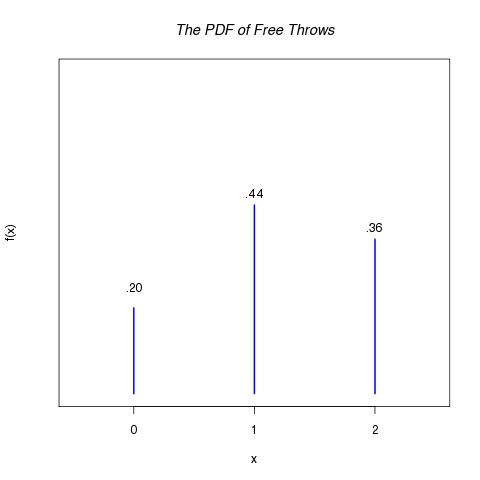
\includegraphics[width=3in]{Larry.jpeg}
\caption{The Probability Density Function of Larry Bird Free Throws}
\end{figure}

\newpage

When dealing with more than two random variables we subscript the PDF's as follows:

\begin{itemize}
 \item $f_{x}$ is the PDF of $X$
 \item $f_{y}$ is the PDF of $Y$
\end{itemize}

\vspace{2mm}

A variable $X$ is a \textbf{continuous random variable} if it takes on any real value with \emph{zero}
probability. A continuous random variable $X$ can take on so many possible values that they are not 
countable, so logical consistency requires that each one has probability zero.

\vspace{2mm}

Examples:

\begin{itemize}
 \item Prices
 \item Wages
 \item Interest rates
 \item Height
 \item Weight
 \item Waiting time
\end{itemize} 





\end{document}


